\documentclass{article}
\usepackage[utf8]{inputenc}
\usepackage{geometry}
\geometry{hmargin=2.5cm,vmargin=2.5cm}
\usepackage{mathtools} %\usepackage{align}
%\usepackage[french]{babel}
\usepackage{graphicx}
\usepackage{bbold}

\title{SOD333 - Rapport}
\author{Paul-Antoine Leveilley \& Mila Rocco}
\date{Septembre 2022}

\begin{document}

\maketitle

\begin{center}

\end{center}

\newpage
\tableofcontents
\newpage





\newpage
\section{TP1: calcul d'une intégrale par méthode de Monte-Carlo, échantillonage préférentiel.}

\subsection{Introduction}

Dans ce TP, on se propose de calculer une intégrale par méthode de Monte Carlo. De manière générale, la méthode de Monte Carlo
consisite à approcher l'intégrale : 
\[I = \int g(x)q(x)dx\] 
Ou q est une densité, par l'estimateur : 
\[\hat{\mu}_N = \frac{1}{N} \sum_{i=1}^N g(X_i)\]

En effet, d'après la loi forte des grands nombres, 
\[\hat{\mu}_N\underset{p.s.}{\longrightarrow}I \]

Pour illustrer cette méthode, nous allons estimer l'intégrale 
\[\int_0^1 cos(\frac{\pi x}{2})dx\]
Dont la valeur se calcule analytiquement, et vaut $\frac{2}{\pi}$

Pour ce faire, on choisit la loi uniforme sur $[0,1]$, qui admet pour densité $q(x) = \mathbb{1}_{x \in [0,1]}$, ainsi que $g(x) = \cos (\frac{\pi x}{2})$

 \subsection{Application "brute" de la Méthode de Monte Carlo}
On décide d'étudier l'échantillon $(X_i)_{1\leq i \leq N}$ , qui suit la loi uniforme sur $[0;1]$ afin de vérifier qu'on estime bien µ avec la méthode de Monte Carlo. Sa fonction de densité est donc $q=U([0;1])$. On choisira $N=50$ pour l'étude empirique du problème.

Pour évaluer µ, on applique la méthode de Monte Carlo, et on obtient l'approximation 
$$\hat{\mu}_N = \frac{1}{N} \sum_{i=1}^N g(X_i)$$

- Calculer la variance théorique\\
\begin{align*} 
  Var(\hat{\mu}_N) &= \frac1{N^2} \sum_{i=1}^N Var(g(X_i))\\ 
  &= \frac1{N^2}\times N Var(cos(\frac{\pi X}2)) \\ 
  &= \frac1{N} \left ( \int_0^1 cos^2(\frac{\pi x}2)dx - \left ( \int_0^1 cos(\frac{\pi x}2)dx \right )^2 \right )\\
  &= \frac1{N} \left ( \int_0^1 \frac{1+cos(\pi x)}{2}dx - 
   \frac4{\pi^2} \right )\\
  &= \frac1{N} \left ( \frac{1}{2} - 
   \frac4{\pi^2} \right )\\
  &\approx \frac{0,095}{N}
\end{align*}

- Estimer empiriquement la variance (prendre N = 50)\\
\textbf{résultats du TP.}
On applique la méthode de Monte Carlo et on en tire un échantillon de $NbMC=1000$ tirages.

\begin{figure}[ht]
\centering
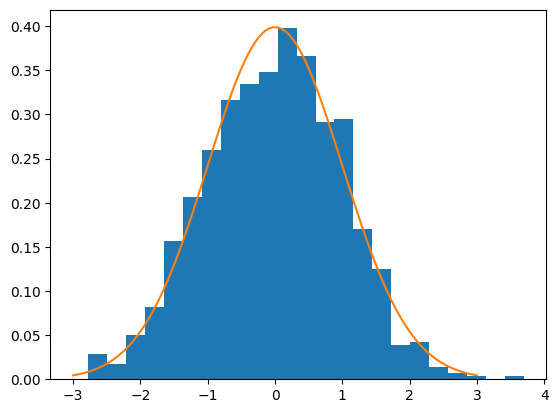
\includegraphics[width=0.4\textwidth]{TP1/MC_brute_TCL.png}
\caption{résultat du TCL}
\end{figure}

\subsection{Echantillonage pondéré}
On génère un nouvel échantillon $(X_i)_{1\leq i \leq N}$ suivant maintenant une fonction d'importance (FI) $\Tilde{q}$ au plus proche de $g(x)$: $X_i \hookrightarrow \Tilde{q}$. Le changement de probabilité donne: 
$$ \hat{\mu}_N = \frac1{N} \sum_{i=1}^N g(X_i)\frac{q(X_i)}{\Tilde{q}(X_i)}\ \overset{p.s.}{\longrightarrow}\ \mu $$

- Chercher une bonne FI\\
(idée: DL au voisinage de 0)  \\
On approxime la fonction g par son développement à l'ordre 2 en 0 (l'ordre 2 ne suffit pas pour que gq et $\Tilde{q}$ gardent le même signe sur $[0,1]$. Rappelons le développement limité en 0 de la fonction cosinus: 
$ cos(x) = 1 - \frac{x^2}{2} + o(x^2) $.
On prend donc pour Fonction d'Importance: 
$$\Tilde{q}_1(x):= 1 - \frac{\pi^2}{8} x^2 $$
Il est important de prendre en compte le fait que $\Tilde{q}$ ne doit pas s'annuler si gq ne s'annule pas. Le DL doit donc être corrigé d'un facteur pour que $\Tilde{q}$ ne devienne pas négatif en $x=1$. En $x=1$, la fonction précédente vaut $\delta = 1 - \frac{\pi^2}{8} < 0$, donc on soustrait $\delta$ à $\Tilde{q}$ pour obtenir notre nouvelle fonction d'importance :
$$\Tilde{q}_2(x):= \frac{\pi^2}{8}(1 - x^2) $$

- Calculer la variance théorique\\
\begin{align*} 
  Var(\hat{\mu}_N) &= \frac1{N^2} \sum_{i=1}^N Var \left ( g(X_i)\frac{q(X_i)}{\Tilde{q}(X_i)}\right)\\ 
  &= \frac1{N} Var\left (\frac{cos(\frac{\pi X}2)}{\frac{\pi^2}{8} (1 - X^2)} \right ) \\ 
  &= \frac1{N} \left ( \int_0^1 \left (\frac{cos(\frac{\pi x}2)}{\frac{\pi^2}{8} (1 -  x^2)} \right )^2dx - \left ( \int_0^1 \frac{cos(\frac{\pi x}2)}{\frac{\pi^2}{8} (1 -  x^2)}dx \right )^2 \right )\\
\end{align*}

\textbf{Application numérique (TP):}

\begin{figure}[ht]
\centering
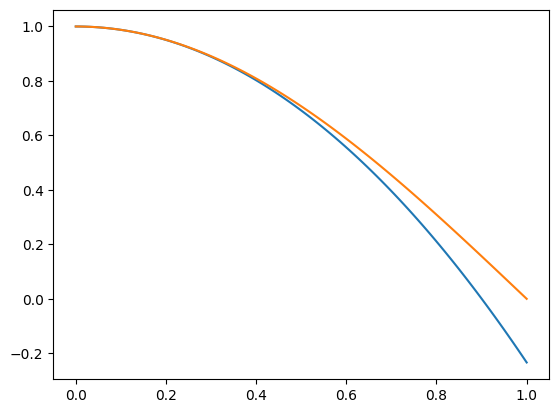
\includegraphics[width=0.4\textwidth]{TP1/DL_ordre2_g.png}
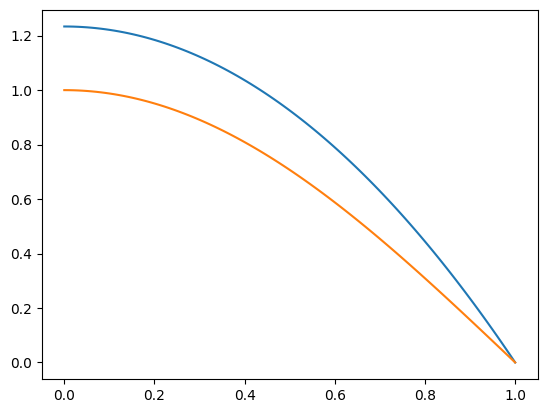
\includegraphics[width=0.4\textwidth]{TP1/DL_ordre2_corrige.png}
\caption{représentation des fonctions gq (en orange) et $\Tilde{q}$ (en bleu): à gauche $\Tilde{q}_1$, à droite $\Tilde{q}_2$}
\end{figure}

\begin{figure}[ht]
\centering
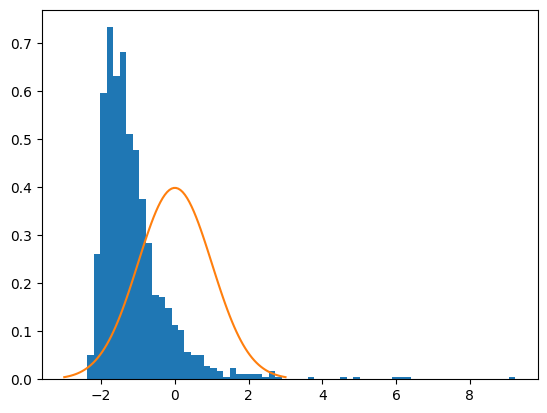
\includegraphics[width=0.4\textwidth]{TP1/IS_TCL_DL_ordre2.png}
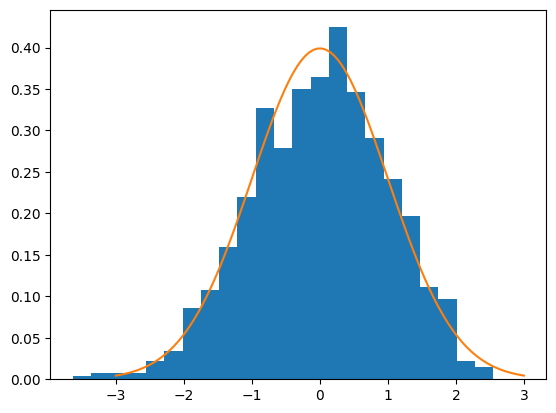
\includegraphics[width=0.4\textwidth]{TP1/IS_TCL_DL_ordre2_corrige.png}
\caption{TCL appliqués respectivement à $\Tilde{q}_1$ (à gauche) et $\Tilde{q}_2$ (à droite)}
\end{figure}

Les résultats du TCL appliqués aux échantillons produits mettent ici en valeur l'importance d'avoir une fonction d'importance du même signe que gq, et que notre développement limité en 0 de gq semble être une bonne approximation pour notre problème.\\

- Utiliser la méthode de rejet pour  générer suivant la FI \\ (Comparer la probabilité d’acceptation théorique à celle obtenue par simulations)\\
On génère un échantillon suivant $p$, et on choisit pour majorant de $g$, $C=1$ tels que 
$$p(x) = \frac{g(x)q(x)}{\int_0^1 g(x)q(x)dx}\ \ \ \ \&\ \ \ \ g(x) \leq C,\ \forall x \in [0;1] $$

Probabilité d'acceptation théorique: 
$$P_a = \frac1C \int_0^1 g(x)q(x)dx 
= \int_0^1 cos(\frac{\pi x}{2})dx 
=\frac{2}{\pi} 
\approx 0,637$$

- Estimer empiriquement la variance.\\
\textbf{application numérique (TP):} On obtient ...

\subsection{Conclusion}
On cherche maintenant à comparer les deux méthodes précédemment appliquées.

- Comparer le rapport des variances des 2 méthodes. Théoriquement et par simulations\\


- Valider par simulations les TCL pour les 2 méthodes en comparant la loi théorique (loi normale) à la loi empirique (histogramme)\\


- Comparer les budgets pour chaque méthode\\


- Calculer la variance de l’estimateur en prenant la FI optimale\\


- Même travail avec $\Tilde{q}=2(1-x)$, ici on simule la FI par la méthode d’inversion de la CDF\\









\newpage
\section{TP2: titre du TP}
\subsection{Introduction}
Dans ce TP, nous allons simuler la trajectoire d'un mobile, et tenter de retrouver ces valeurs grâce à des observations que nous aurons de sa trajectoire.

\begin{figure}[ht]
\centering
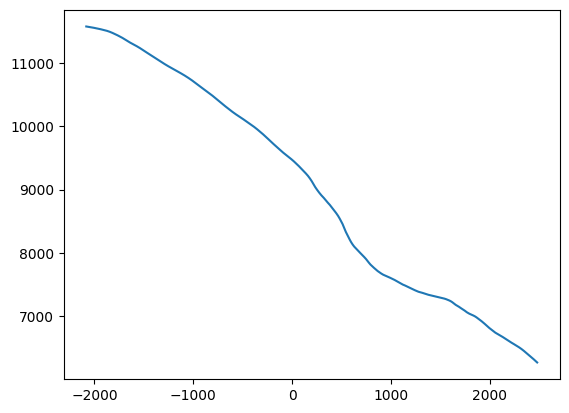
\includegraphics[width=0.4\textwidth]{TP2/position_réelle.png}
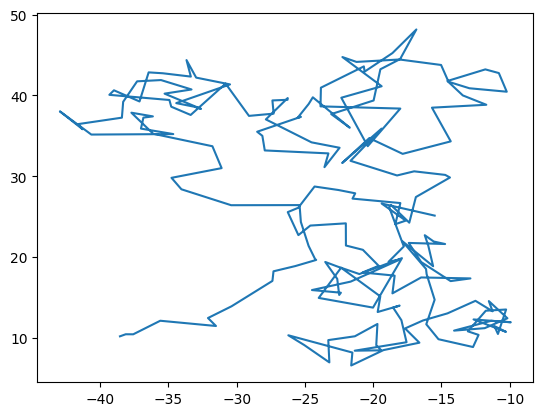
\includegraphics[width=0.4\textwidth]{TP2/vitesse_reelle.png}
\caption{Trajectoire et vitesse associée, que l'on cherche à retrouver}
\end{figure}

\subsection{Titre intermédiaire}
\subsection{Conclusion}

\newpage
\section{TP3 : Borne de Cramer Rao.}
\subsection{Introduction}
\subsubsection{Formulation du problème}

Dans ce TP, on se propose de calculer une borne de Cramer Rao pour un problème de filtrage. Le cadre général est le suivant.
On se donne un système  $(X_{k})_{k\geq 0}$ sujet à une certaine dynamique,
ainsi qu'une série de mesures bruitées $(y_{k})_{k \geq 0}$ (bruit gaussien de variance $\sigma_{k}^{2}$) : 
\[\left\{\begin{array}{ll}
   X_{k+1} = \phi(k,k+1)X_{k} \\
   y_{k}=h_{k}(X_{k})+\epsilon_{k}
\end{array}\right. \]

Avec $X_{0} \sim  \mathcal{N} (X_{\nu},P_{0})$. On peut montrer que la matrice d'information ralative à l'instant $k$ vérifie
la relation de récurence suivante : 

\[ J_{k} = \frac{1}{\sigma_{k}}\left(\frac{\partial h_{k}}{\partial X_{k}}\right)\left(\frac{\partial h_{k}}{\partial X_{k}}\right)^{T}+\left(\frac{\partial X_{k-1}}{\partial X_{k}}\right)^{T}J_{k-1}\left(\frac{\partial X_{k-1}}{\partial X_{k}}\right)\]

Avec $J_{0}=P_{0}^{-1}$ et $\phi(k,k+1)=\frac{\partial X_{k+1}}{\partial X_{k}}$.
La borne de Cramer Rao à l'instant $k$ est alors égale à l'inverse de la matrice d'information : 
\[BCR_{k}= J_{k}^{-1}\]

Nous étudions le système suivant : un bateau émetteur de bruit se déplace dans le plan de manière rectiligne uniforme. 
Un bateau observateur mesure la direction d'ou lui parvient le bruit, plus précisément, il mesure l'angle $\theta_{k}$ que fait cette direction avec l'horizontale, ce toute les secondes pendant 100s. Le bateau observateur se déplace également en ligne droite à vitesse constante.
L'état de l'émeteur est donné par sa position et sa vitesse : $X_{k} = (x_{k},y_{k},\dot{x}_{k},\dot{y}_{k})$, sa matrice de transition est :
\[\phi(k,k+1) = \phi =  \begin{pmatrix}
  1 & 0 & T & 0 \\
  0 & 1 & 0 & T \\
  0 & 0 & 1 & 0 \\
  0 & 0 & 0 & 1 
  \end{pmatrix}\]

Pour pouvoir discriminer entre différentes
trajectoires possibles, le bateau doit virer de bord à un certain moment. En effet on peut vérifier que s'il ne le fait pas, des trajectoires différentes peuvent donner lieu à des mesures d'angle identiques.
Pour simplifier l'étude, on suppose que le bateau vire de bord toujours au même moment : au milieu du trajet; à l'instant $k = 50s$. Le bateau observateur choisit l'angle $\varphi $ duquel il tourne. Chaque choix de $\varphi$ 
conduit à une précision différente de l'estimation de la trajectoire  de l'émeteur.
La question est donc la suivante : quel choix de $\varphi$ est le meilleur pour estimer la trajectoire de l'émeteur?
\\
Pour répondre à cette question, nous allons simuler la dynamique de l'éméteur et de l'observateur. Grâce à ces dynamiques, nous allons
calculer le gradient de la fonction d'observation et nous allons en déduire la matrice d'information.
Dans notre cas, la fonction d'observation est l'angle que fait la direction d'observation avec l'horizontale. 
En terme de l'abscisse et de l'ordonnée de l'éméteur et de l'observateur, cette fonction s'écrit : 
\[\theta_{k} = h_{k}(X_{k})=\arctan \left(\frac{y_{k}-y_{k}^{o}}{x_{k}-x_{k}^{o}}\right)\]

En inversant la matrice d'observation, on obtiendra la borne de Cramer Rao, sous forme d'une matrice carrée d'ordre 4.
On cherchera ensuite la valeur de $\varphi$ qui minimise le critère : $\sqrt{\sigma_{x_{n}}^{2}+\sigma_{y_{n}}^{2}}$

\subsubsection{Calcul du gradient de $h_{k}$ par rapport à $X_{k}$}
Déjà, on voit facilement que : 
\[\frac{\partial h_{k}}{\partial \dot{x}_{k}} = 0 \] et :
\[\frac{\partial h_{k}}{\partial \dot{y}_{k}} = 0 \]
Ensuite, par le calcul, on a que : 
\[\frac{\partial h_{k}}{\partial x_{k}}=\frac{y_{k}^{o}-y_{k}}{\left(x_{k}-x_{k}^{o}\right)^{2}\left(1+\left(\frac{y_{k}-y_{k}^{o}}{x_{k}-x_{k}^{o}}\right)^{2}\right)}\]
et :

\[\frac{\partial h_{k}}{\partial y_{k}}= \frac{1}{\left(x_{k}-x_{k}^{o}\right)\left(1+\left( \frac{y_{k}-y_{k}^{o}}{x_{k}-x_{k}^{o}}  \right)^{2}\right)}\]
\subsection{Simulations des dynamiques de l'observateur et de l'émetteur}
Nous avons simulé la dynamique du système pour différents changements de cap de l'observateur, avec les paramètres du tableau \ref{paramètres}.
 Nous obtenons les tracés de la figure \ref{trajectoire}


\begin{figure}[h!]
  \centering
  \caption{Paramètres pour la simulation}
  \label{paramètres}
  \begin{tabular}{|*{11}{c|}}
    \hline Horizon temporel & $T = 1$ \\
    \hline Nombre de mesures  & $N=100$ \\
    \hline Ecart type du bruit & $\sigma_{k}=1^{\circ}$\\
    \hline Vitesse de l'observateur & $V_{o}=10 m.s^{-1}$\\
    \hline Position initiale de l'observateur &  $(x_{0}^{o},y_{0}^{o})=(0,0)$ m\\
    \hline Vitesse de l'émetteur & $V_{e} = 5 m.s^{-1}$\\
    \hline Cap de l'émetteur & $\alpha =-20^{\circ}$\\
    \hline Position initiale de l'émetteur & $(x_{0},y_{0})=(2000,2000)$\\
    \hline Incertitude initiale sur la position de l'émetteur & $P_{0}=diag(1000,1000,10,10)^{2}$\\
    \hline
  \end{tabular}
\end{figure}


 \begin{figure}[h!]
  \centering
  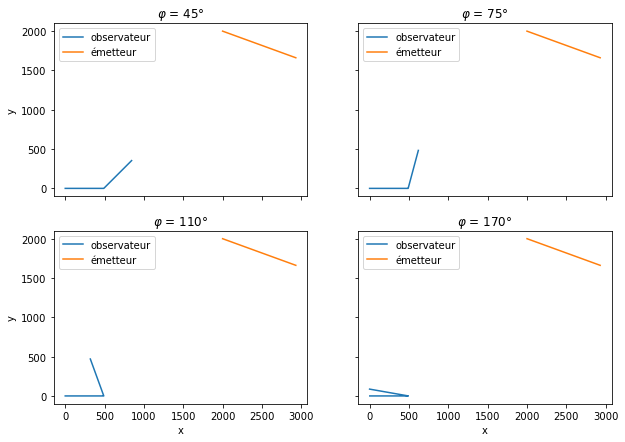
\includegraphics[width = 15cm]{TP3/trajectoires.png}
  \label{trajectoire}
  \caption{Trajectoires de l'émetteur et de l'observateur pour différentes valeurs de l'angle $\varphi$}
\end{figure}

Grâce à ces dynamiques, nous sommes capables de calculer la Borne de Cramer Rao associée à cet estimateur de la position de l'émetteur. 
Nous présentons ces résultat en figure \ref{cramerrao}. 

\begin{figure}[h!]
  \centering
  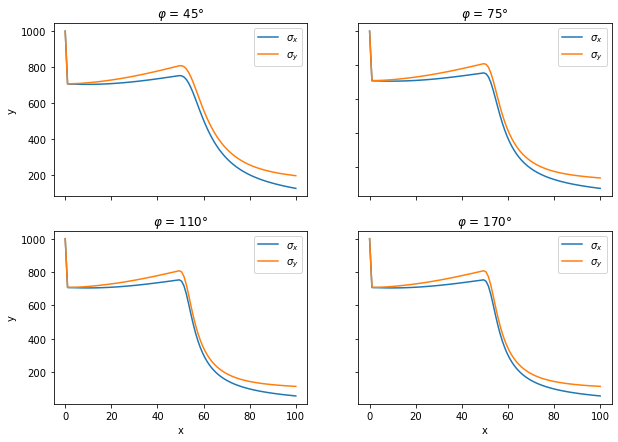
\includegraphics[width = 15cm]{TP3/cramer rao.png}
  \caption{Borne de Cramer Rao pour l'abscisse et l'ordonnée de la position de l'émetteur au cours du temps, pour différentes valeurs de $\varphi$}
  \label{cramerrao}
\end{figure}

\subsection{Optimisation de la valeur de $\varphi$}
Pour trouver la valeur de $\varphi$ optimale, nous avons simplement testé toutes les valeurs entre $0^{\circ}$ et $360^{\circ}$, avec un pas de 
$1^{\circ}$. Nous avons trouvé une valeur optimale de $\varphi = 109^{\circ}$, ce qui correspond à la trajectoire représentée en figure
\ref{optimale}. La borne de Cramer Rao associée est représentée en figure \ref{crameropti}. Le critère associé est un écart type sur la position de 128m.
\begin{figure}
  \centering
  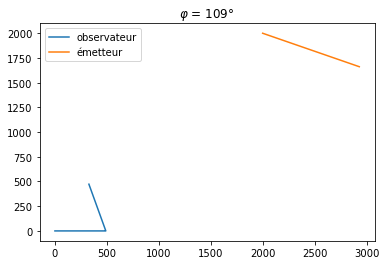
\includegraphics[width = 10 cm]{TP3/trajopti.png}
  \label{optimale}
  \caption{Trajectoire optimale pour l'observateur}
\end{figure}

\begin{figure}
  \centering
  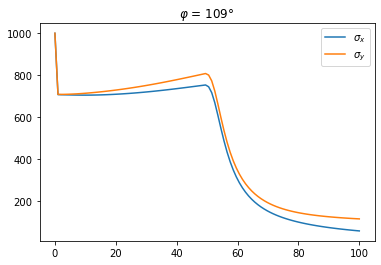
\includegraphics[width = 10 cm]{TP3/crameropti.png}
  \label{crameropti}
  \caption{Borne de Cramer Rao pour la trajectoire optimale}
\end{figure}

\subsection{Conclusion}
En conclusion, ce TP nous aura permis de voir comment la Borne de Cramer Rao permet de réaliser le choix d'une stratégie pour 
optimiser la précision sur l'estimation de état d'un système, grâce à la seule connaissance d'un modèle à priori.
\newpage
\section{TP4: titre du TP}
\subsection{Introduction}
\subsection{Titre intermédiaire}
\subsection{Conclusion}

\end{document}
